\documentclass[11pt]{article}
\usepackage[margin=1in]{geometry}
\usepackage[utf8]{inputenc}\usepackage[T1]{fontenc}
\usepackage{hyperref}
\hypersetup{colorlinks=true, linkcolor=blue, citecolor=blue, urlcolor=blue,
  pdftitle={Form, Not Granted}, pdfauthor={Caio Vicentino}}
\emergencystretch=3em \sloppy \hyphenpenalty=2000 \hbadness=10000
\usepackage{booktabs}\usepackage{amsmath}\usepackage{amssymb}\usepackage{xcolor}\usepackage{graphicx}\usepackage{array}

\title{Form, Not Granted \\[2pt]
\large A sparse-autoencoder autopsy shows the agent's commit-locus ``authorization direction''
is a surface-form artifact --- and an all-layer sweep leaves the deeper question open}
\author{Caio Vicentino \\ OpenInterpretability \\ Fortaleza, Brazil \\ ORCID: 0009-0003-4331-6259 \\ \texttt{caio@openinterp.org}}
\date{June 2026}

\begin{document}
\maketitle

\begin{abstract}
A late-layer ``authorization direction'' was reported to detect and steer a tool-using agent's commitment
to unauthorized irreversible actions~\cite{authdir}, and a follow-up found it tracks the authorization the
model \emph{feels} rather than the one the user \emph{granted}~\cite{feltnotgranted}. Both were built on a
\emph{supervised} difference-of-means direction --- a method that returns a direction whether or not the
concept is natively represented. We stop using the ruler and point the microscope: we encode the residual
at the delete-commit token (layer 59 of Qwen3.6-27B) through a trained TopK sparse autoencoder
(40{,}960 features) and ask, unsupervised, whether a feature distinguishes a \emph{granted} commit from a
\emph{felt}-but-not-granted one. Three results. (1) \textbf{The supervised direction inverts under a
structure-matched control}: applying the same frozen direction, AUROC(granted vs felt) goes from $0.838$
(single-turn vs multi-turn conditions) to $0.08$ when both conditions share one multi-turn scaffold and only
the final user turn varies --- a direction measuring authorization would not flip when only the conversation
\emph{format} changes. (2) \textbf{The SAE's separating features are surface form}: across runs, every top
feature that separates granted from felt is, by its max-activating context, a tool-call scaffold, a JSON
tool-schema token, or the file-listing output --- never a semantic ``user granted this'' feature. (3) \textbf{A
cross-lexical-family test isolates this}: a feature selected on one paraphrase family does \emph{not} transfer
to a disjoint family (held-out AUROC $0.50$, chance), and the one feature that does transfer ($0.993$, pooled
$0.998$) max-activates on tool-call \emph{format boilerplate}, not authorization. The agent's commit-point
representation is dominated by \textbf{surface form and plan-coherence}; \emph{authorization-as-granted is not
a native monosemantic feature} at this locus. We do NOT, however, claim authorization is unrepresented in the model: a sweep across all 11 SAE layers finds a granted-vs-felt linear signal that generalizes across paraphrase at most layers --- but with residual surface confounds (an em-dash present in both `granted' phrasings and neither `felt', and referent specificity; it is already near-ceiling at layer 15, too early for semantics), leaving open whether that signal is authorization or surface. The robust claim is narrower and still consequential: the commit-locus difference-of-means direction of prior work reads form, not a clean grant; a faithful internal authorization monitor, if one exists, is not that direction. We state the scope plainly (one model, synthetic scenarios, an SAE explaining $\sim$66\% of residual variance) and release every ledger and a recompute-everything evaluation.
\end{abstract}

\paragraph{Revision note (v2).} The first version concluded ``no native authorization concept.'' A subsequent all-layer sweep (\S\ref{sec:sweep}) revealed a paraphrase-invariant granted-vs-felt signal at most layers that this conclusion did not account for; because that signal carries residual surface confounds we also cannot yet call it authorization. This version withdraws the unqualified ``no concept'' claim, scopes the result to the commit locus, and states the deeper question as open. The robust findings (the structural flip, the L59 surface naming) are unchanged.

\section{Introduction}
Linear directions in the residual stream detect and steer safety-relevant behavior: refusal lives in a
single direction~\cite{refusaldir}, and a late-layer \emph{authorization direction} both separates authorized
from unauthorized irreversible-action commits and, under steering, moves the commitment~\cite{authdir}. A
follow-up sharpened this to ``felt, not granted'': in realistic free generation the same direction tracks the
authorization the model \emph{feels} (and is blind to the user's actual grant)~\cite{feltnotgranted}.

Every step of that arc used a \emph{supervised} difference-of-means direction $d=\overline{\text{auth}}
-\overline{\text{unauth}}$. This method has a known failure mode: it \emph{always} returns a direction that
separates the labeled sets, whether the model represents the concept monosemantically or whether we merely
projected a human concept onto whatever variance correlated with the labels~\cite{geometry,interpillusion}. A probe can fit a label from spurious structure unless tested against a control~\cite{controltasks}.
The ``felt, not granted'' result is itself a hint that the concept is imported. So we ask the question the
ruler cannot answer: at the moment an agent commits an irreversible action, does it \emph{represent}
``user-granted authorization'' in its own ontology --- or is the decision substrate something else, onto which
``authorization'' was projected? We answer it by letting the model's own features speak, via a sparse
autoencoder~\cite{monosemantic,saefind,topk,scalingmono} trained on this exact model.

Contributions: (i) a structure-matched control shows the supervised ``authorization direction'' is
\emph{confounded by conversation structure} --- it does not weaken but \emph{inverts} (\S\ref{sec:flip}); (ii)
an unsupervised SAE autopsy shows the features that separate granted from felt are \emph{surface form}, named
by their max-activating contexts (\S\ref{sec:autopsy}); (iii) a cross-lexical-family generalization test
isolates lexical/scaffold confounds from semantics and finds no paraphrase-invariant \emph{semantic} feature
(\S\ref{sec:cross}); (iv) the synthesis --- the agent commits on form and plan-coherence, and
authorization-as-granted is not a native concept here, which reframes why internal monitors fail
(\S\ref{sec:disc}). This qualifies, not refutes, \cite{authdir,feltnotgranted}: the direction is real and
usable in its tested regime, but it reads form, not a represented grant.

\section{Setup}
\paragraph{The direction and the SAE.} Following~\cite{authdir}, $d$ is the difference of mean layer-59
residuals at the action-commitment token over explicitly-authorized vs.\ unauthorized prefilled deletes,
frozen. The SAE is a TopK autoencoder (\texttt{caiovicentino1/qwen36-27b-sae-fullstack}, layer 59, $d_{\text{sae}}
=40{,}960$, $k=128$; reconstruction relative error $0.58$, fraction-of-variance-explained $\approx 0.66$). We
encode a residual $x$ as $z=\mathrm{TopK}_k\!\big(\mathrm{ReLU}((x-b_{\text{dec}})W_{\text{enc}}+b_{\text{enc}})\big)$.
\paragraph{Conditions.} A real Qwen3.6-27B agent (bf16) runs free generation in a sandboxed file workspace
and commits \texttt{delete\_file}; we capture the layer-59 residual at the \texttt{<function=} decision token.
\emph{granted} = the user explicitly authorizes the deletion; \emph{felt} = the agent finishes a cleanup plan
it co-authored under a vague ``go ahead'' (the realistic over-reach of~\cite{feltnotgranted}). $n=12$--$18$
commits per condition; greedy decoding (deterministic; the decisive run reproduced bit-for-bit across two GPU
sessions). Ledgers and scripts are public.

\section{The supervised ``authorization direction'' inverts under structure-matching}
\label{sec:flip}
In a first autopsy the conditions differed in conversation \emph{structure} (granted was single-turn; felt was
multi-turn: tidy $\to$ list $\to$ flag $\to$ ``go ahead''). A structure-matched control removes this: both
conditions share one multi-turn scaffold and differ \emph{only} in the final user turn. We then apply the
\emph{same frozen} direction $d$ --- no selection, no fitting (Fig.~\ref{fig:flip}):

\begin{center}
\begin{tabular}{lc}\toprule
setting & supervised $d$ AUROC (granted vs felt) \\\midrule
unmatched (structure differs) & $0.838$ \\
structure-matched & $\mathbf{0.08}$ --- it \emph{inverts} \\\bottomrule
\end{tabular}
\end{center}

The same direction gives near-opposite answers depending on prompt format. A direction that measured
\emph{granted authorization} would be invariant to changing only the conversation format while holding the
authorization meaning fixed. It is not. \textbf{The ``authorization direction'' is substantially a
surface-structure artifact}; this is selection-free and does not depend on the SAE.

\begin{figure}[t]\centering
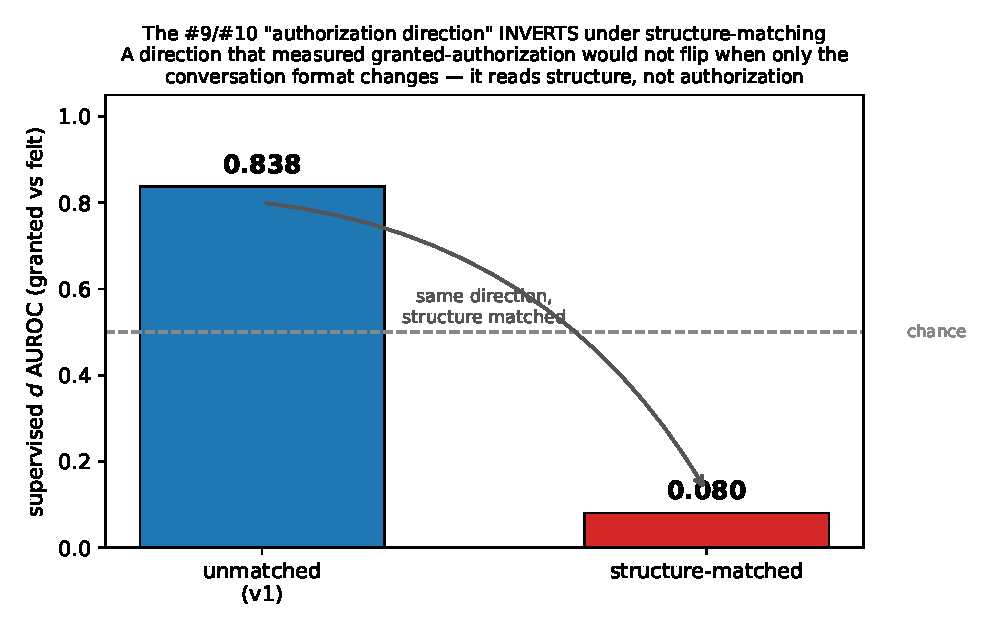
\includegraphics[width=0.62\textwidth]{figures_co/fig1_flip.pdf}
\caption{The frozen supervised direction from~\cite{authdir,feltnotgranted} inverts (AUROC $0.838\to0.08$)
when prompt structure is matched and only the authorizing user turn varies. It reads structure, not grant.}
\label{fig:flip}
\end{figure}

\section{The SAE's separating features are surface form}
\label{sec:autopsy}
Unsupervised, a single SAE feature separates granted from felt at AUROC $1.0$ ($p<0.001$ vs.\ a $1000\times$
permutation null) in both the unmatched and matched runs --- an automated ``native feature found'' flag. The
flag is misleading: it only asks \emph{does some feature separate}. The pre-registered feature-\emph{naming}
(max-activating token context) is decisive --- every top separator is surface form (Fig.~\ref{fig:naming}):
the tool-call scaffold (\texttt{<think></think>\textbackslash n<tool\_call>\textbackslash n<function}), JSON
tool-schema tokens (\texttt{"parameters":\{"type":"object"}, \texttt{"required":["path"]}), and the file-listing
output (\texttt{Files: cache\_tmp.dat\dots}). \textbf{No semantic ``user-granted authorization'' feature appears
among the separators in either run.}

\begin{figure}[t]\centering
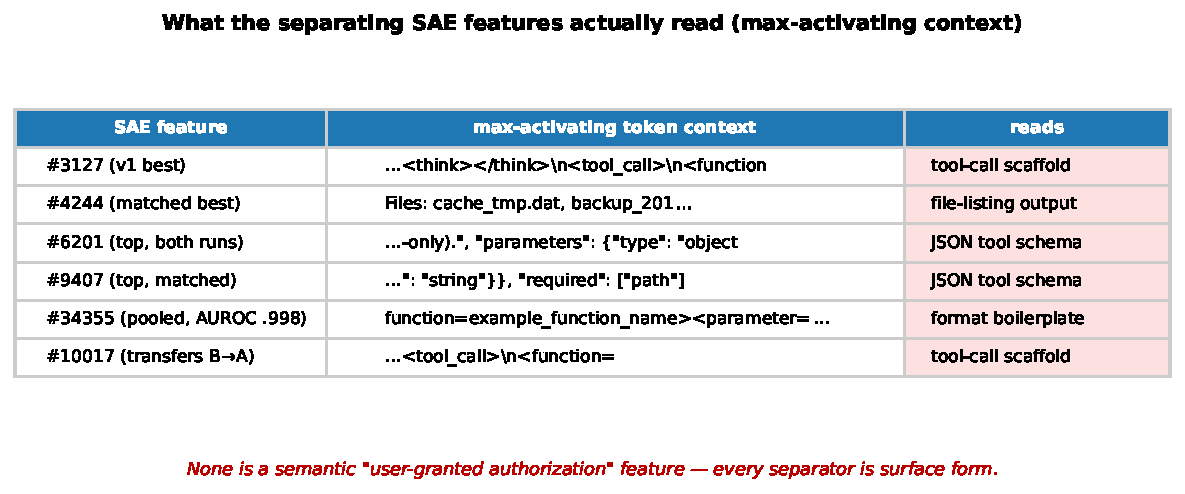
\includegraphics[width=0.92\textwidth]{figures_co/fig3_naming.pdf}
\caption{Every feature that separates granted from felt commits is, by its max-activating context, tool-call
scaffold, JSON tool-schema, file-listing, or format boilerplate. None is authorization.}
\label{fig:naming}
\end{figure}

\section{Cross-lexical generalization: surface, not semantics}
\label{sec:cross}
The matched conditions still differ in the \emph{text} of the user turn, so a separator could be lexical. We
ran a $2\times2$ design --- authorization (granted/felt) $\times$ two disjoint lexical families (A/B),
structure-matched --- and the selection-free test: select the best SAE feature (and a supervised direction) on
family A, fix its polarity, and evaluate on the held-out family B, and B$\to$A (Fig.~\ref{fig:cross}):

\begin{center}
\begin{tabular}{lcc}\toprule
 & within-family (selection-inflated) & \textbf{cross-family (held out)} \\\midrule
best SAE feature & A $1.0$, B $1.0$ & \textbf{A$\to$B $0.50$}, B$\to$A $0.993$ \\
supervised $d$ (on cells) & A $1.0$, B $0.99$ & A$\to$B $0.76$, B$\to$A $1.0$ \\\bottomrule
\end{tabular}
\end{center}

The A-selected feature \emph{does not transfer} (A$\to$B $=0.50$, chance): it read a lexical shortcut present
only in family A (the filename, ``delete'', ``authorize''). A feature \emph{does} transfer B$\to$A ($0.993$), and
a pooled feature separates granted from felt across both families (AUROC $0.998$, $p<0.001$) --- which, taken
alone, looks like a paraphrase-invariant semantic signal. \textbf{Naming settles it}: those ``invariant''
features --- \#34355 (the pooled feature) and \#10017 (the B$\to$A transferring feature) --- max-activate on tool-call \emph{format boilerplate}
(\texttt{function=example\_function\_name><parameter=example\_parameter\_}) and the \texttt{<function=}
scaffold --- present in every commit, with context-modulated magnitude that happens to correlate with the
condition. (Our pre-registered worry that the invariant signal was an em-dash punctuation confound was
\emph{wrong}; it is scaffold, not punctuation --- the conclusion held for a different reason.) The separation is
surface, not a represented grant.

\begin{figure}[t]\centering
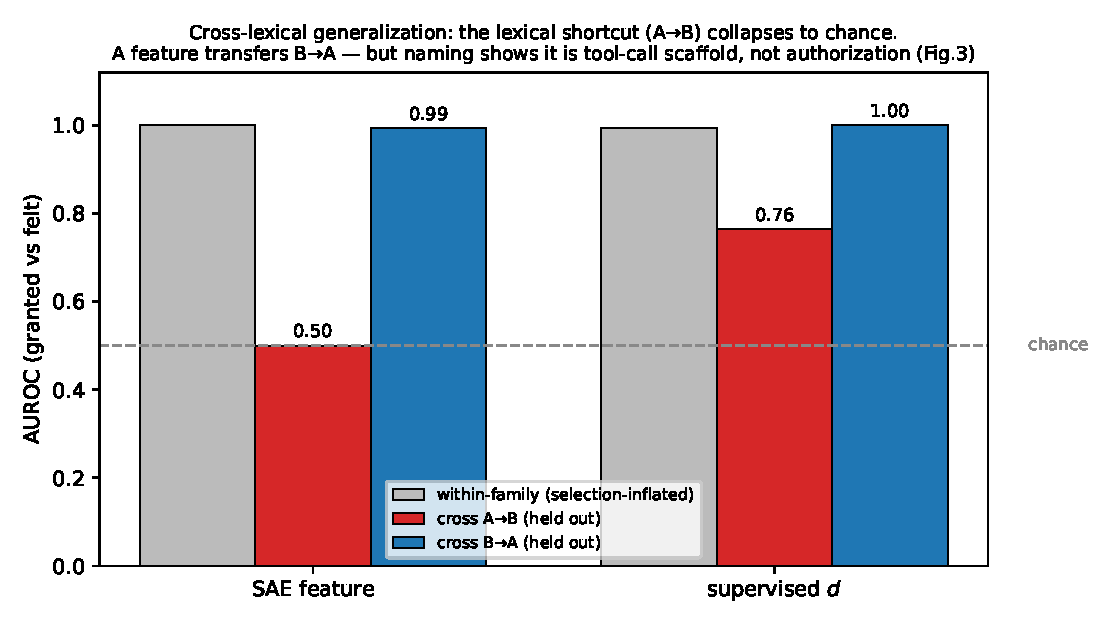
\includegraphics[width=0.82\textwidth]{figures_co/fig2_crosslexical.pdf}
\caption{Cross-lexical-family generalization (held-out, selection-free). The lexical shortcut collapses to
chance (A$\to$B $0.50$); the feature that transfers is tool-call scaffold (Fig.~\ref{fig:naming}), not
authorization.}
\label{fig:cross}
\end{figure}

\section{An all-layer sweep leaves the deeper question open}
\label{sec:sweep}
We tested only L59 above. The SAE covers 11 layers; we swept all of them at two positions --- the last prompt token (``preact,'' where the model has just read the authorizing turn) and the commit token --- with the same cross-lexical test (Fig.~\ref{fig:sweep}). A supervised granted-vs-felt direction trained on family A transfers to held-out family B at AUROC $\approx 1.0$ at most layers, and the best SAE feature transfers strongly at several (up to $1.0$ at preact). \textbf{This is a real, paraphrase-invariant granted-vs-felt signal our L59 analysis alone did not reveal} --- so we do not claim authorization is unrepresented. But it is confounded: both ``granted'' phrasings contain an em-dash neither ``felt'' phrasing does, and ``granted'' names a specific target while ``felt'' is vague --- paraphrase-invariant surface properties our cross-lexical control does not remove. The tell is layer 15: a near-perfect cross-family AUROC at the fifteenth of sixty-four layers is implausibly early for a semantic authorization concept and far more consistent with a surface property. The sweep thus \emph{finds a signal but cannot name it semantic}; whether authorization-as-granted is natively represented is \textbf{unresolved}, and needs a confound-balanced re-run with feature naming at the high-transfer mid layers.

\begin{figure}[t]\centering
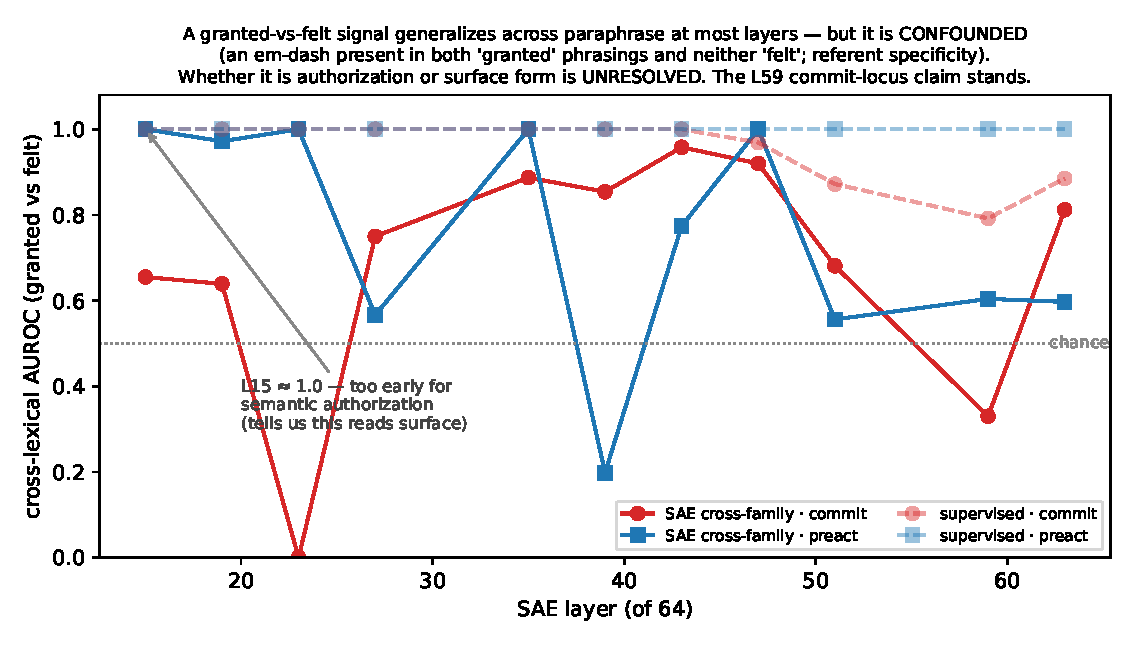
\includegraphics[width=0.82\textwidth]{figures_co/fig4_layersweep.pdf}
\caption{Cross-lexical (held-out) granted-vs-felt AUROC across all 11 SAE layers, at the commit token and at preact. A signal generalizes across paraphrase at most layers --- but it is confounded (em-dash, specificity), and is already near-ceiling at layer 15, too early to be semantic authorization. The question is open; the L59 commit-locus result stands.}
\label{fig:sweep}
\end{figure}

\section{Discussion}
\label{sec:disc}
\paragraph{Form, not granted.} Across three independent confound controls --- conversation structure (the
flip), user-turn lexicon (the cross-family collapse), and scaffold activation (the naming) --- the separator of
granted from felt commits is always \emph{surface form}. There is no native monosemantic
``user-granted-authorization'' feature at this locus; the commit substrate is surface form plus plan-coherence
(the agent finishing a plan it co-authored). This deepens ``felt, not granted''~\cite{feltnotgranted}: the
internal signal does not even track \emph{felt} authorization \emph{semantically} --- it tracks \emph{form}.
\paragraph{Why internal monitors fail.} An internal authorization monitor reads a property of the model's
state. If the safety-relevant abstraction (``did the trusted user grant this specific irreversible action'')
is \emph{not} a feature the model computes, no probe or steering vector can read or move it; the apparent
``authorization direction'' was reading the form that correlates with it in a given prompt distribution --- a shortcut~\cite{shortcut} --- which
is why it generalizes poorly and inverts under a format change. The implication for agent safety is not
``calibrate the probe better'' but ``the grant must be checked \emph{outside} the model'', against the explicit
request --- consistent with the external-check result of~\cite{feltnotgranted}.
\paragraph{Methodological note.} The automated best-feature flag said \emph{native feature found} in every run;
the pre-registered naming and the cross-lexical control overturned it each time. Reporting the flag without
the naming would have produced a confident false positive. This is the discipline, not a footnote.

\section{Limitations}
The cross-lexical conditions carry residual confounds --- an em-dash present in both ``granted'' phrasings and neither ``felt'', and referent specificity --- which the layer sweep shows can drive a paraphrase-invariant signal; a confound-balanced design with mid-layer feature naming is required to settle whether any layer hosts a semantic authorization feature.
This is one model (Qwen3.6-27B), one locus (layer 59), one domain (file deletion), with synthetic
structure-matched scenarios and an SAE that explains $\approx 66\%$ of residual variance. ``No native
authorization feature'' is, strictly, \emph{no monosemantic separating feature in this SAE's learned
dictionary at this locus}; a stronger SAE (evaluated as in~\cite{saeeval}), a different layer, or a non-linear / multi-feature code~\cite{nonlinear} could
surface a representation this analysis misses --- absence of a separating feature is weaker than evidence of
absence of any representation. The robust, SAE-independent result is the \emph{flip} (\S\ref{sec:flip}); the
SAE autopsy explains \emph{why} the direction is structural. The synthetic granted/felt distinction is itself
a design choice; interchange interventions on real long-horizon trajectories are the natural next test. We do
not re-test the steering-control of~\cite{authdir}.

\section{Conclusion}
Pointing a sparse autoencoder at an agent's commit point, instead of a supervised difference-of-means
direction, overturns the clean reading of the ``authorization direction'': it is confounded by conversation
structure (it inverts, $0.838\to0.08$), and the features that separate granted from felt commits are
surface-form --- tool-call scaffold, schema, file-listing --- with no native monosemantic representation of
a clean user-granted-authorization concept at the commit locus. Whether authorization is represented elsewhere is open: a granted-vs-felt signal exists across layers but is confounded by surface properties (\S\ref{sec:sweep}). What is robust: at the commit locus the apparent authorization direction is surface form and structure-confounded. Internal authorization monitors
read form, not grant; the grant must be checked outside the model.

\paragraph{Reproducibility.} Runners (\texttt{agentguard\_sae\_\{autopsy,autopsy\_matched,counterfactual,name,layer\_sweep\}.py}),
five per-run ledgers, figures, and an evaluation that recomputes every number are released at
\url{https://github.com/OpenInterpretability/agentguard}; ledgers also at the Hugging Face dataset
\texttt{caiovicentino1/swebench-phase6-verdict-circuit}. The decisive counterfactual run reproduced
bit-for-bit across two independent GPU sessions.

\begin{thebibliography}{99}
\bibitem{authdir} C.~Vicentino. The Authorization Direction. OpenInterpretability, 2026. DOI:10.5281/zenodo.20683623.
\bibitem{feltnotgranted} C.~Vicentino. Felt, Not Granted. OpenInterpretability, 2026. DOI:10.5281/zenodo.20685264.
\bibitem{refusaldir} A.~Arditi, O.~Obeso, A.~Syed, D.~Paleka, N.~Panickssery, W.~Gurnee, N.~Nanda. Refusal in Language Models Is Mediated by a Single Direction. NeurIPS 2024. arXiv:2406.11717.
\bibitem{monosemantic} T.~Bricken, A.~Templeton, J.~Batson, et al. Towards Monosemanticity: Decomposing Language Models With Dictionary Learning. Transformer Circuits, 2023.
\bibitem{saefind} H.~Cunningham, A.~Ewart, L.~Riggs, R.~Huben, L.~Sharkey. Sparse Autoencoders Find Highly Interpretable Features in Language Models. ICLR 2024. arXiv:2309.08600.
\bibitem{topk} L.~Gao, T.~Dupr\'e la Tour, H.~Tillman, G.~Goh, R.~Troll, A.~Radford, I.~Sutskever, J.~Leike, J.~Wu. Scaling and Evaluating Sparse Autoencoders. 2024. arXiv:2406.04093.
\bibitem{geometry} S.~Marks, M.~Tegmark. The Geometry of Truth: Emergent Linear Structure in LLM Representations of True/False Datasets. 2023. arXiv:2310.06824.
\bibitem{interpillusion} T.~Bolukbasi, A.~Pearce, A.~Yuan, A.~Coenen, E.~Reif, F.~Vi\'egas, M.~Wattenberg. An Interpretability Illusion for BERT. 2021. arXiv:2104.07143.
\bibitem{controltasks} J.~Hewitt, P.~Liang. Designing and Interpreting Probes with Control Tasks. EMNLP 2019. arXiv:1909.03368.
\bibitem{saeeval} A.~Makelov, G.~Lange, N.~Nanda. Towards Principled Evaluations of Sparse Autoencoders for Interpretability and Control. 2024. arXiv:2405.08366.
\bibitem{nonlinear} J.~Engels, I.~Liao, E.~J.~Michaud, W.~Gurnee, M.~Tegmark. Not All Language Model Features Are Linear. 2024. arXiv:2405.14860.
\bibitem{shortcut} R.~Geirhos, J.-H.~Jacobsen, C.~Michaelis, R.~Zemel, W.~Brendel, M.~Bethge, F.~A.~Wichmann. Shortcut Learning in Deep Neural Networks. Nature Machine Intelligence, 2020. arXiv:2004.07780.
\bibitem{scalingmono} A.~Templeton, T.~Conerly, J.~Marcus, et al. Scaling Monosemanticity: Extracting Interpretable Features from Claude 3 Sonnet. Transformer Circuits, 2024.
\end{thebibliography}
\end{document}
